\begin{comment}
Template vir elke funksie
    \paragraph{Funksie naam}
			\begin{description}
			    \item{\textbf{Priority}:} %watter prioriteit dit het: Critical, Important of Nic-to-have
			    \item{\textbf{Service Contract}:}% Wat dit doen
			    \item{\textbf{Pre-conditions}:}%wat moet waar wees voor die funksie sy ding kan doen
    			    \begin{itemize}
    			        \item %precondition 1
    			        \item %precondition 2
    			    \end{itemize}
			    \item{\textbf{Post-conditions}:} % wat moet waar wees na die funksie sy ding gedoen het
    			    \begin{itemize}
    			    \item %post condition 1
    			    \item %post condition2
    			    \end{itemize}
			\end{description}
\end{comment}








	\subsection{Server}
	    \subsubsection{Scope: }
	    \begin{itemize}
	    \item The server is used with the gateway: it sends and receives data to and from the server. 
	    \item A user can add, remove and edit meetings on the server via the website.
	    \item A user can add people to a meeting and remove people from a meeting on the server via the website.
	    \item The server stores a database with all the data.
	    \end{itemize}

%		\begin{figure}[H]
 %			 \centering
%			  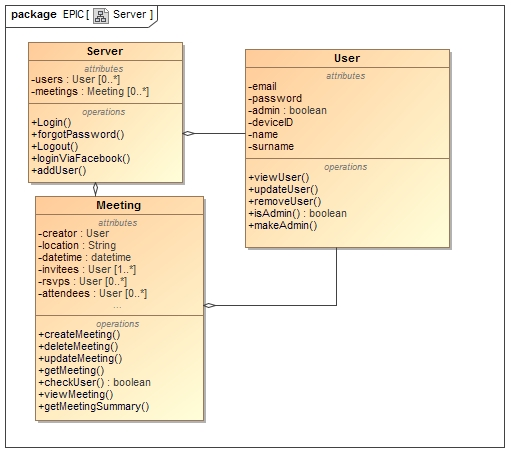
\includegraphics[width=12cm]{ServerClass}
%		 	 \caption{A Class Diagram of the Server}
%		\end{figure}
		
		
		
		\subsubsection{Functionality}
		
		    \paragraph{getMeeting}
			\begin{description}
			    \item{\textbf{Priority}:} Critical%watter prioriteit dit het: Critical, Important of Nic-to-have
			    \item{\textbf{Service Contract}:} A query is made for a specific meeting and the function returns a JSON object with the meeting that meet the query. 
			    \item{\textbf{Pre-conditions}:}%wat moet waar wees voor die funksie sy ding kan doen
    			    \begin{itemize}
    			        \item The query must be valid.
    			        \item The meeting must exist.
    			    \end{itemize}
			    \item{\textbf{Post-conditions}:} % wat moet waar wees na die funksie sy ding gedoen het
    			    \begin{itemize}
    			    \item A meeting object that meet the query is returned. 
    			    \item The action is logged on the server.
    			    \end{itemize}
			\end{description}
	

		    \paragraph{getPeopleList}
			\begin{description}
			    \item{\textbf{Priority}:} Critical%watter prioriteit dit het: Critical, Important of Nic-to-have
			    \item{\textbf{Service Contract}:} This function returns a list of Person object that may attend a specified meeting.
			    \item{\textbf{Pre-conditions}:}%wat moet waar wees voor die funksie sy ding kan doen
    			    \begin{itemize}
    			        \item The meeting must be specified.
    			        \item The meeting must exist.%precondition 1
    			        \item Only the owner of the meeting or the gateway may call this function. \item The server must be running.%precondition 2
    			    \end{itemize}
			    \item{\textbf{Post-conditions}:} % wat moet waar wees na die funksie sy ding gedoen het
    			    \begin{itemize}
    			    \item A list of Person objects is returned.%post condition 1
    			    \item The action is logged.%post condition2
    			    \end{itemize}
			\end{description}
			

    \paragraph{Create Person}
			\begin{description}
			    \item{\textbf{Priority}:} Critical %watter prioriteit dit het: Critical, Important of Nice-to-have
			    \item{\textbf{Service Contract}:} This function is called when a person is added to a meetings people list and the person is not yet in the database. The function creates a Person object and stores it in the database.
			    \item{\textbf{Pre-conditions}:}%wat moet waar wees voor die funksie sy ding kan doen
    			    \begin{itemize}
    			        \item The user must have permission to add the person.
    			        \item The required fields are email address, name and surname.
    			    \end{itemize}
			    \item{\textbf{Post-conditions}:} % wat moet waar wees na die funksie sy ding gedoen het
    			    \begin{itemize}
    			    \item The person object is created and it is added to the database.
    			    \item The action is logged in the database.
    			    \end{itemize}
			\end{description}
    

    \paragraph{Create meeting}
			\begin{description}
			    \item{\textbf{Priority}:} Critical%watter prioriteit dit het: Critical, Important of Nic-to-have
			    \item{\textbf{Service Contract}:} The function is called by the website when the user creates a meeting. The meeting object is then created and stored in the database.% Wat dit doen
			    \item{\textbf{Pre-conditions}:}%wat moet waar wees voor die funksie sy ding kan doen
    			    \begin{itemize}
    			        \item The meeting title, meeting room, date and time are required fields.
    			    \end{itemize}
			    \item{\textbf{Post-conditions}:} % wat moet waar wees na die funksie sy ding gedoen het
    			    \begin{itemize}
    			    \item The meeting object is created and it is added to the database.
    			    \item The action is logged in the database.
    			    \end{itemize}
			\end{description}
